\documentclass[12pt,a4paper,notitlepage]{report}
\usepackage[utf8]{inputenc}
\usepackage{cite}
\usepackage{etoolbox}
\usepackage{listings}
\usepackage{graphicx}


%%%%%%%% Bibliografi %%%%%%%%%%%%%%%%%%%%%%%%%%%%%%%%%
%% Ändrar namnet på referens headern
\renewcommand\bibname{References (Vi har URL och Datum, måste bara ändra LaTeX layouten.)}
%% Ser till att referenserna kommer på en egen sida och att titeln inte är numrerad
\makeatletter
\patchcmd{\thebibliography}{%
  \cleardoublepage
  \chapter*{\bibname}\@mkboth{\MakeUppercase\bibname}{\MakeUppercase\bibname}}{%
  \section{References}}{}{}
\makeatother
%%%%%%%%%%%%%%%%%%%%%%%%%%%%%%%%%%%%%%%%%%%%%%%%%%%%%%

%%%%%%%%%%%%%%%%% Start document %%%%%%%%%%%%%%%%%%%%%
\begin{document}
\title{Report Draft\\Digitalization of Visual Acuity Testing}
\author{Anders Ohlsson\\Christian Johansson\\Svante Nilsson}
\maketitle

\begin{abstract}
Digitalization of Visual Acuity Testing is a project involving development of a method for displaying optician's eye charts. The charts are going to be displayed on a digital screen and controled via an Android tablet. This solves several problems relating to lighting and distance from the patient to the chart, while also providing more ways for the optician to tailor the examination of the patient. The Digitalization of Visual Acuity Testing project will be improving upon a proof-of-concept system that has been used to test whether or not digital screens are a viable alternative to physical charts.
\end{abstract}
\thispagestyle{empty}
\clearpage

\tableofcontents
\thispagestyle{empty}
\clearpage

%%%%%%%%%%%%%%%%%%%%%%%%  DEL 1: FÖRUTSÄTTNINGAR
\setcounter{page}{1}
\chapter{Preconditions}
%%%%%%%%%%%%%Område/bakgrund: vilket är området, omgivningen, kontextet, bakgrunden för projektet? beskrivning av området (t.ex. ljudbehandling, studieplaner, visualisering, autism...)
\section{Background}
\subsection{Visual Acuity}
To measure a patients visual acuity opticians today use charts with printed lines of continuously smaller symbols. The measurement is made by having the patient read symbols on the chart from a set distance. The person reads down the chart until it is no longer possible to make out the characters. Based on the size of the character the patient failed to recognize, a visual acuity can be determined. 

For such charts to function as a basis for these standardized tests of visual acuity the testing environment must be carefully prepared. Among a few things, for the measurement to be optimal the chart must be placed at a distance of six meters from the patient, and the luminosity in the room must be at a specific level. In the event that the room is too small or the lighting insufficient, this can lead to irregularities or faulty measurements in some tests. 

These conditions cannot always be met. Sometimes the examination room is not sufficiently large for measurements from six meters. In the event that the room is too small or the lighting insufficient, this can lead to irregularities or faulty measurements in some tests. % Skriv mer om varför det måste vara tillräckligt mycket ljus. Referens behövs.

There are also several different variations on these charts. Different sets of symbols, ranging from different subsets of latin letters to more abstract symbols, have been developed for different types of patients, such as those who are analphabetic, or for small children. The layout of these charts also have variations, from the classic Snellen Chart that was developed in the 19th century, to the more modern LogMAR chart.

\section{Related work}
Several pieces of software exists that tries to solve the problems of displaying information from an android tablet or phone on a larger screen. 

\subsubsection{Chromecast and Apple TV}
The Chromecast \cite{chromecast} and Apple TV \cite{appletv} are small devices which are plugged into a TV and enables mobile phones and tablets to stream media to them. The devices are small and easy to handle and a lot of applications support streaming to them. The Chromecast is specifically made for android devices and Apple TV for iOS device, but they both support each other.

\subsubsection{Digital Eye Chart}
 Digital Eye Chart \cite{digitaleyechart} is a visual acuity testing program that attempts to solve the problem of having several charts by using a monitor instead. The user can then, with the help of a computer, change the symbols on the chart and even generate a random chart. 

\subsubsection{iChart+}
iChartPlus \cite{ichartplus} is another program which is similar to Digital Eye Chart but also have an adjustable viewing distance. 

\subsubsection{AxAnIvIs}
AxAnIvIs is a prototype that is currently under testing at Uppsala University Hospital. The project attempts to improve on how we perform visual acuity tests by digitalizing them. It adds more types of charts than the standard physical ones that exists today. The system uses a webbrowser running on an android tablet that is connected to a screen. A library of vector graphic files are displayed in the webbrowser. These files contains the different charts as well as some other specialized tools. Currently the android tablet has to be held in a fixed position in the examination room, restrained by the cable going to the screen. The charts used are fixed and not very easily changed, which makes it very hard to try out new techniques and methods of measuring.

\subsubsection{Our project}
Most of the before mentioned systems have some form of negative side that we try to improve on, mostly problems about high cost and difficulties with extending the software. We are different with that we want to create a system that is cheap, easy to understand and easy to maintain. Creating a system that have all the previously mentioned sides is one of the goals we have. Another important goal is creating a system that really is speacialized on measurements of visual acuity. All these points are important to give the users the best experience.

\section{Purpose}
The purpose of this project is to remove the constraints of using physical charts for visual acuity tests and instead use a screen or monitor that can change optotypes and sizes with the press of a button.

\subsection{Problem}
The problem with today's visual acuity tests are that they are very clumsy to work with. The charts are printed and contains only one type of symbol, or optotype. This could be letters for people with the ability to read or an 'E' shape turned in different ways which allows children who are unable to read, or illiterate people, to identify which symbol they see. These charts are also only designed to be viewed from one specific distance, which makes some rooms to small and unusable.

\subsection{Advantages of a digital system}
The advantages of a digital system is the ability to change the layout, optotypes and size of the chart without having to carry away the old chart and then carrying back a new. This will save both time and space as only one screen and a small Android device is necessary. This system will also allow the visual acuity tests to take place in rooms that previously where too small, as the system will display optotypes at a size suitable for the distance the patient is from the monitor.

\subsection{Disadvantages of a digital system}
A disadvantage with this system is that digital screens become very expensive at large sizes, which limits the maximum distance a patient can sit from the screen. Another disadvantage is that the resolution, or rather pixel density, will limit how close to a screen a patient can sit without the optotypes looking pixelated. Pixel density is a measurement of how many pixels (dots) can fit in a small section of the screen, usually denoted as Pixels Per Inch (PPI) or Dots Per Inch (DPI). The higher the DPI is the better the quality of small details will be. This is very important when rendering type fonts because the edges should be as smooth as possible.

%\section{Employer}
%%%%%%%%%%%%%beskriv uppdragsgivare, om ni har

%Vår uppdragsgivare är Per Söderberg, professor i oftalmiatrik vid Institutet%(Institutionen?)<---------------------------------- 
%för Neurovetenskap vid %Hum. Dubbel-vid. Hur skriver man det här egentligen? <---------------------------------------------------
%Uppsala Universitet. Han tar även patienter vid Akademiska Sjukhuset i Uppsala

%Our employer is Per Söderberg, professor and chair of opthalmology with the Department of Neuroscience at Uppsala University. He also takes patients at the university hospital, and uses these types of charts on a daily basis. 

%%%%%%%%%%%%%%%%%%%%%%%%Syfte: vart strävar projektet? vad är det övergripande målet, nyttan, effekterna av projektet?
%%%%%%%%%%%%%t.ex. bättre koll på kosthållning, enklare planering av studier
\section{Purpose (Should be removed or changed)}
To solve the problems with this system the Department of Neuroscience have performed tests using a digital screen to present the charts instead of using printed medium. This means the optician can have many more variations on the charts at disposal. The set of symbols used on the charts can be switched with a menu, and the screen provides an adequately lit surface by itself. The current system is implemented by connecting an android tablet to a screen via an HDMI cable, and the charts are rendered via a web browser on the tablet. Testing has proceeded for over a year, and has yielded very good results.

The goal of this project is to take the system used for these tests and develop a complete implementation with several advantages over the testing system, such as:

\begin{itemize}
	\item A fully developed app for the tablet with an improved user interface, both aesthetically and mechanically.
	%\item Connecting the digital screen to a computer that can handle higher resolution rendering than the tablets native resolution.
	\item Controlling the computer over WiFi using the tablet, meaning the optician can move around the room more easily.
	\item Altering the scale of the rendered symbols so that the patient can be closer or further away from the screen than the regular six meters.
	\item Being able to tailor the testing process to the patient by changing the sets of symbols displayed or removing clutter from the charts.
\end{itemize}
	
and other features to make the process easier for the optician and patient.

%%%%%%%%%%%%%%%%%%%%%%%%Mål: vad ska konkret levereras/utföras av projektet, för att ta oss närmare syftet

%Hum. Ta material från ovanstående fråga? Jag är inte säker.

%%%%%%%%%%%%%%%%%%%%%%%%Motivation:
\section{Motivation}
This project is important because determining visual acuity is a very labor- and equipment-intensive process. As the testing has showed, using a digital chart with a tablet interface is easier and faster, and can be a great help for the optician. The only thing missing is to improve on the design and implement a functional user interface and a better hardware solution to turn the testing shell into a finished product. 

%Borde utökas, trorja.
%%%%%%%%%%%%%%%%%%%%%%%%Lägesbeskrivning:

%Fan också, det här har jag ju skrivit om redan. 
%Att upprepa sig, eller inte upprepa sig. Det är frågan.

%%%%%%%%%%%%%vad vet ni om läget när det gäller "problemet" som projektet ska lösa?
%%%%%%%%%%%%%vilka andra har försökt lösa det, eller gjort relaterade/liknande saker/system? Referera.

%Man kan ju också prata i mer detalj om Snellen och LogMAR... Men det är ju egentligen inte information som är viktig för oss. 

%%%%%%%%%%%%%%%%%%%%%%%%Frågeställningar:

\section{Issues} %vilka tekniska problem behöver ni lösa (sj.arb), vad ska ni ta reda på (uppsatsmetodik)?
There are several technical problems that we need to solve. We need to design a small computer system that will store and present the desired images to the screen. Our current plan is using a RaspberryPi, since it is a cheap and compact alternative to PCs that is more than powerful enough for our purposes. Though, since the RaspberryPi in running on a ARM CPU there will be a few compatibility problems that we need to solve. For example is the Java graphics library JavaFX, that is going to replace the older Swing library, not very well supported by RaspberryPi. Not being able to use the latest features can create problems in the future when some things get deprecated. Though if that happens it is probably not very hard to re-write the GUI to a supported JavaFX version.

Networking needs to be added to control the RaspberryPi over WiFi from the tablet, and some features like waking the screen as the app is started can be considered. With networking we face a few problems. % How the server is controlled by the tablet? (Direct function calls, network polling, blabla)

Designing the android app for the tablet will bring technical problems, both from the limitations of portable computers, and making our software adaptable enough to work on as many brands of tablets as possible. For example, the symbols we are to present are stored in the .svg (Scalable Vector Graphics) format, which is not natively supported on android. Because of this we must find and work with a licensed third-party software library to render them. Other than that the android tablet doesn't impose too many big problems. %% Fler problem som kan uppstå med android?

Finally we should design a way for the database of symbols and chart layouts to be easily updated and synchronized between devices and some server storage. This will be the least important task for us since it we wan't to focus on having something to work with firstly. Updating and synchronizing can be done by hand locally.

\section{Ethical considerations} %vilka etiska frågeställningar finns (tänk t.ex. på användningen av resultatet)?
Our ethical obligations with this project is providing a functional and stable product. If our system does not perform to specification, a lot of patients could get erroneous measurements during testing, costing a lot of time and money to correct. This is very important to think about since we are dealing with treatment of people.

\chapter{Problem Description}

\chapter{Theory}

\section{Choice of distance} %% Nån bra titel här?

The specific distance of six meters is derived from how our eyes bend light. From a distance of six meters the rays of light seem to be nearly parallel to eachother. % Borde skriva mer utförligt? Referens behövs.
It is important that the rays of light that hit the eyes are parallel because then the light focuses on the same spot in the back of the eyes, which in turn makes the measuring a lot easier and accurate. \cite{PGSoderberg} % Detta kanske ska flyttas till teori delen?

To make up for the shift in focus in the eyes a plus glass has to be put in front of the patients eyes. The glass will bend the light in such a way that the rays of light becomes more parallel. 

\begin{figure}[ht!]
\centering
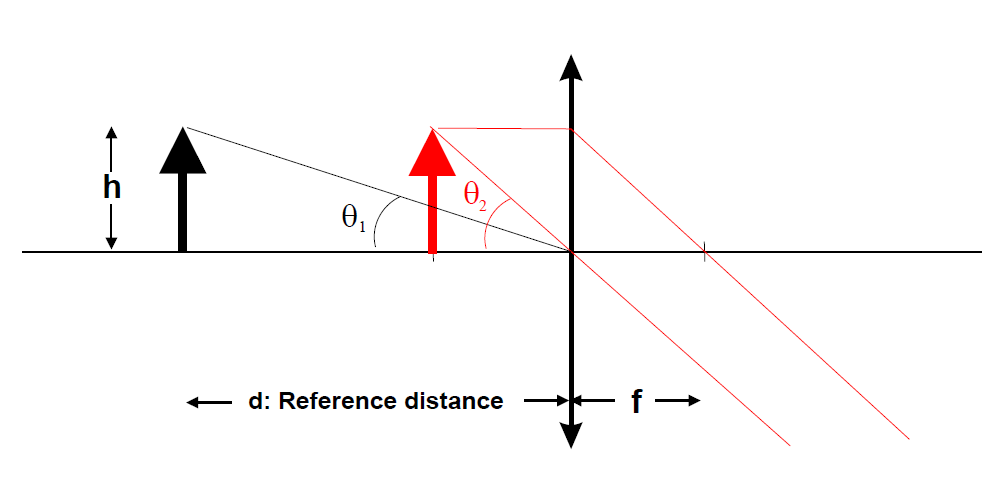
\includegraphics[width=120mm]{images/Angular_magnification.png}
\caption{Angular magnification\label{theory}}
\end{figure}

%%%%%%%%%%%%%%%%%%%%%%%%DEL 2: GENOMFÖRANDE
\chapter{Implementation}

%\section{Methods}



%\subsection{Methods}
%The screen controller will be built using Java and a few third-party libraries. Java has many built-in and well supported packages, and is also mostly platform independent. This suits our needs for future extensions of the system. Since the server mostly handles rendering of images having a good method of displaying images is needed. 

%Thankfully Java offers a few well-known libraries for rendering graphics. For many years the choice has been a now somewhat aged library called Swing \cite{Java_Swing}. Another library, JavaFX, has started to gather people's interests again. This because of the new version released with Java 8, JavaFX 8 \cite{JavaFX_8}. 

%Though it is common to use the newer JavaFX instead of Java Swing, JavaFX is not well supported on the machine we are going to use. Using Java Swing is then a better choice for our project, but if JavaFX becomes better supported in the future it will be easy to re-create our system using JavaFX.

%\subsection{Client application}
%The Android application is written in java, which is the official language for Android. The static parts of the GUI, which will never change unless an application update is released, is written in xml. This is similar to how html is written and is supported by Android natively.

%The charts are generated at runtime and the code is a slightly modified copy of the code used to draw the charts on the server. If the charts would have been written in xml, there would be no guarantee that they would fit on the screen or keep the correct proportions on different tablets. This also avoids hard to read code as the large chart, for example, would need 70 defined areas for images, all with an unique text string id. As Android does not have support for vector graphics and the chart optotype images are vector images the AndroidSVG \cite{AndroidSVG} library is used to display them.

%The settings associated to each chart are also generated at runtime. If this were not the case, every different version of the chart would need its own xml file, as each version contains a different number of predefined charts.

\section{Methods}


%\subsection{Server application}
%The server application is modeled after after the MVC (Model-View-Controller) pattern, where the Model is the logic and the view is GUI (graphical user interface). The server applications controller would be the networking, but for this project the networking was decided to fall outside of the MVC pattern and be its own structural part instead.

%The logic part of the server application is responsible for handling all calculations and data. It contains information about the connected screen and provides methods for getting pixel densities and converting physical measurements, like centimeters, to digital measurements like pixels. The most important part is the method for calculating the correct sizes for the optotypes that should be displayed.

%It is also contains methods for calculating the correct sizes of the optotypes and the data about the charts that should be displayed.


\subsection{Android application}
The Android application is written in java, which is the official language for Android. The static parts of the GUI(graphical user interface), which will never change unless an application update is released, is written in xml. This is similar to how html is written and is supported by Android natively.

The charts shown on the Android device are generated at runtime. If the charts would have been written in xml, there would be no guarantee that they would fit on the screen or keep the correct proportions on different tablets. This also avoids hard to read code as the large chart, for example, would need 70 defined areas for images, all with an unique text string id. As Android does not have support for vector graphics and the chart optotype images are vector images the AndroidSVG \cite{AndroidSVG} library is used to display them.

The settings associated to each chart are also generated at runtime. If this were not the case, every different version of the chart would need its own xml file, as each version contains a different number of predefined charts.

In order to control the application, \textit{controllers} where created in order to listen to button clicks and gestures when the user is attempting to to something.

\subsection{Server application}
The server application is also written in java and uses the built in Swing library for drawing graphics. As most the servers only job is to display charts, almost all code are copied and slightly modified from the Android application. Everything graphical in the server is generated at runtime as the sizes and distances between optotypes depends on which screen that's connected and the distance from the screen to the patient. The PC version of java doesn't support the AndroidSVG library, another vector graphics library called Batik SVG Toolkit \cite{Batik} was used.

\subsection{Network}
The communication between the client and the server consists of two parts. The first part is server detection and the second is server communication. All network communications are handled in threads separate from the main thread as the network operations would halt the flow of the program otherwise. Once the operations are complete and the main threads finds it convenient, it will grab the result from the network threads.

\subsubsection{Server detection}
In order to detect all servers on the network, the Android application sends out a UDP (User Datagram Protocol) broadcast message containing server discovery request. The application will then listen for incoming server responses. Once the application haven't received anything for three seconds from the last server response, it will stop listening and determine that all available servers have responded. The names and addresses of the servers will then be extracted from each response message and stored in a list so the user can choose which one to connect to.

The servers themselves are constantly listening for broadcasts containing the server discovery request. Once a request is received, the server will send a response and then keep listening for more requests.

\subsubsection{Server communication}
The communication between the client and server is handled using simple TCP (Transimission Control Protocol) messages. The TCP messages are used for sending and receiving commands and are structured as three lines of text (Example \ref{tcp_message}). The first line is a \textit{check} word and is the same for every \textit{command}. The second line is a \textit{command} word which tells the receiver what to do and the third line is the \textit{data} required for the \textit{command}. In many cases the simple \textit{command} is enough and the \textit{data} is left empty.

\begin{center}
\renewcommand{\lstlistingname}{Example}
  \lstset{%
    title=Example of TCP message,
    basicstyle=\ttfamily\footnotesize\bfseries,
    xleftmargin=.2\textwidth, xrightmargin=.2\textwidth
  }
\begin{lstlisting}[caption=TCP Message, label=tcp_message]
CHECK_WORD
LARGE_CHART
NULL
\end{lstlisting}
\end{center}


\section{System Structure}
The system is divided into three major parts, an Android application, a server and networking. The Android application and server is modeled after the MVC (Model-View-Controller) pattern, where the model is the logic and the view is the GUI. The controller part is the part on the Android application that listens for button clicks and gestures. Usually the networking would fall under controller in the MVC pattern but was, in this system, chosen to be a separate larger structure.

\begin{figure}[ht!]
\centering
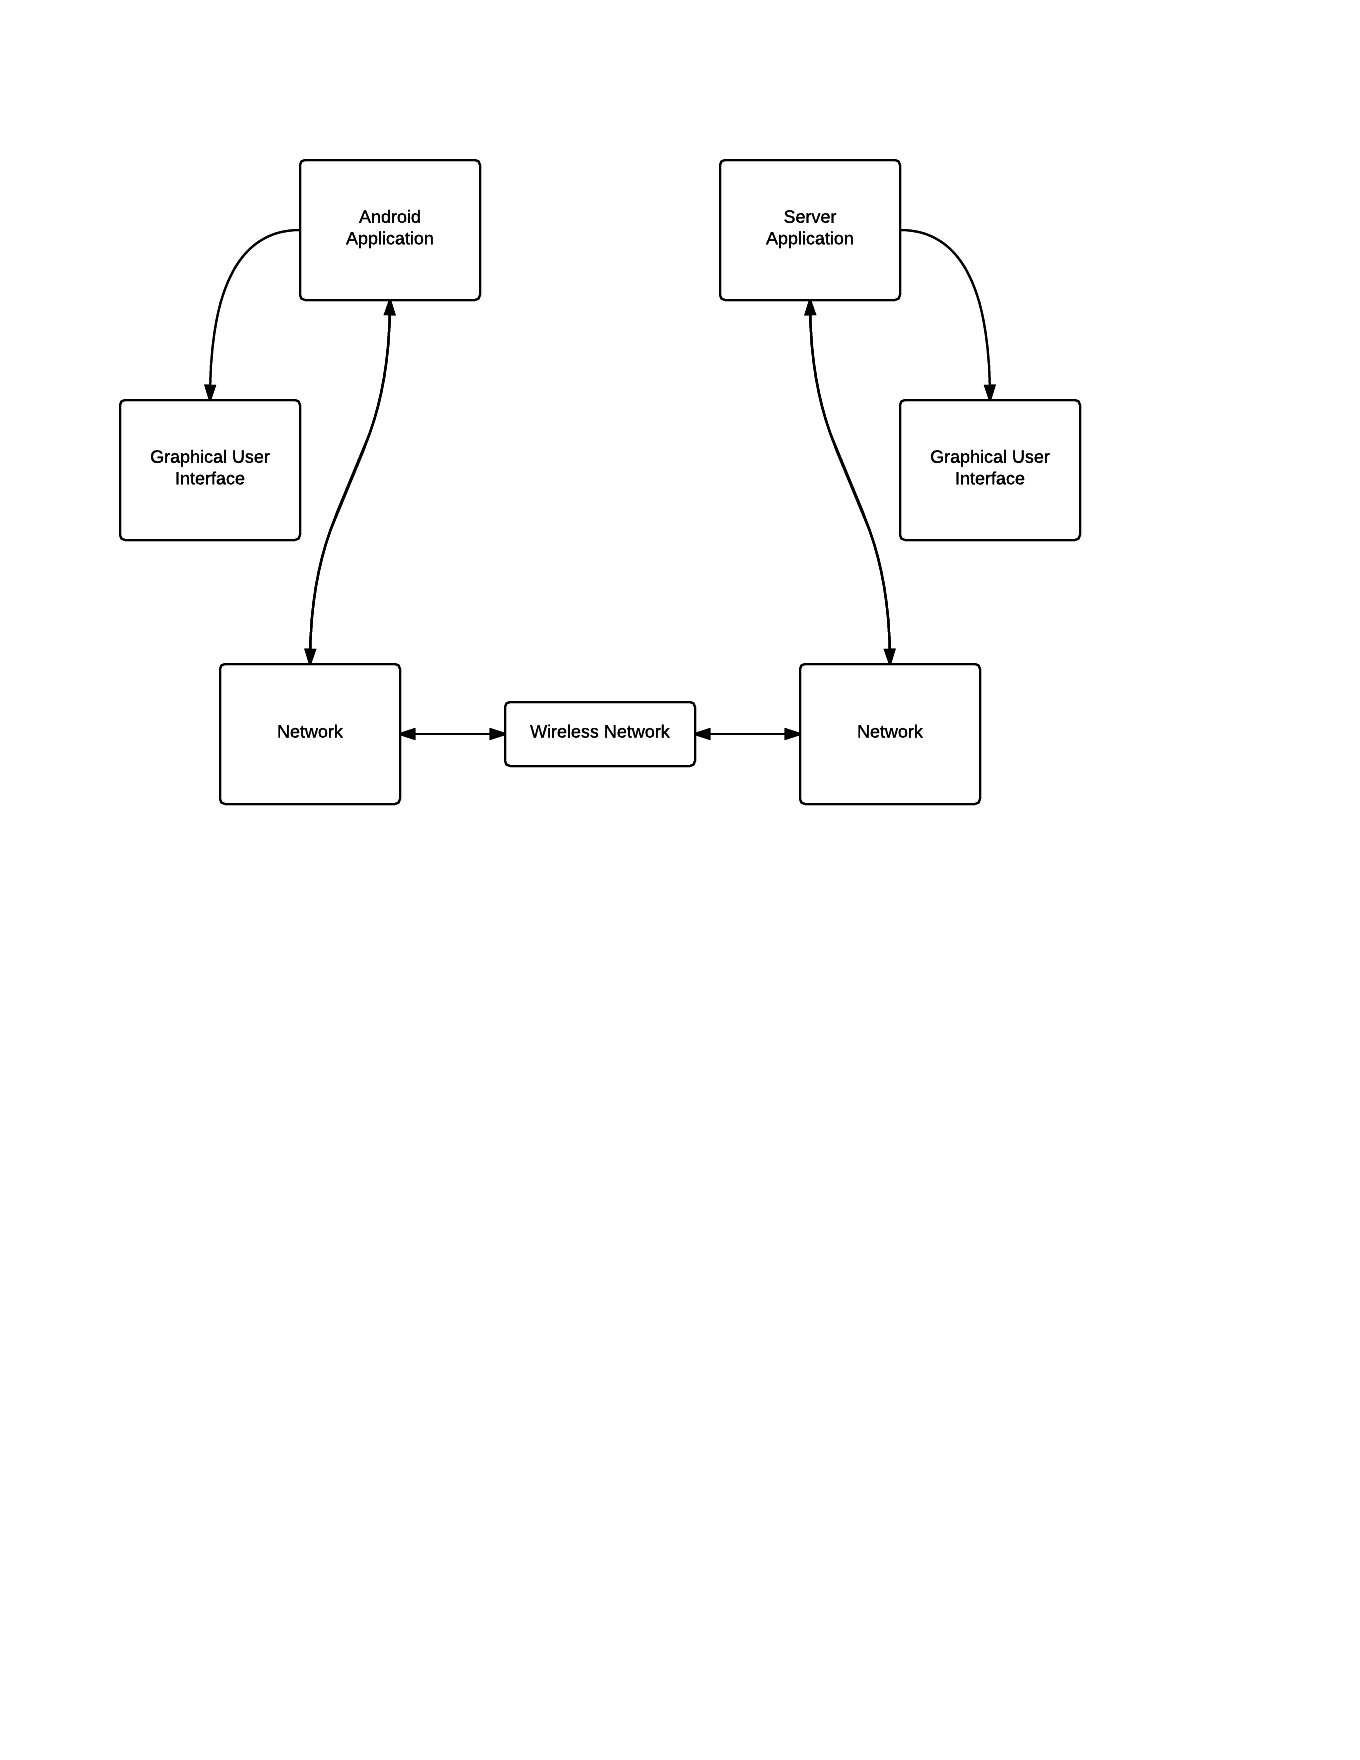
\includegraphics[width=120mm]{images/system_structure.png}
\caption{Overview of the system structure\label{system_structure}}
\end{figure}

 %where the server is connected to a large screen and is controlled by the Android application over a local network. The server and


%The communication between the android tablet and the server will be handled using a third-party network library called Kryonet \cite{Kryonet}. 

%\section{System structure} %%%%%%%%%%%%%%%%%%%%%%%%Systemstruktur: vilka delar kan ni se att ert system/problem består av? (T.ex. databas, webbinterface, AI-modul, grafik...)
%The system is split up between an Android application and a PC application. These applications will both be structured with the Model-View-Controller design pattern as a base in order to split up user input, graphics and logic. The PC application will act as a server and display an eye chart on a larger screen connected with an HDMI-cable. The android applications purpose is to control the PC-application over a wifi network and make sure the correct chart is displayed on the larger screen. The android application will display the same image shown on the large screen, but with some other extra information that's useful for the optician.

%\textbf{Image of System structure TBI}

%The dicrete parts of this project are:

%\begin{itemize}
%	\item Android application
%	\begin{itemize}
%		\item User Interface
%		\item Backend/Network
%	\end{itemize}
%	\item Screen controller
%	\begin{itemize}
%		\item Display
%		\item Backend/Networking
%	\end{itemize}
%\end{itemize}

\section{Boundaries}
%%%%%%%%%%%%%%%%%%%%%%%%Avgränsningar: vad ska INTE göras, även om man kanske kunde tro det?
We are not tasked to develop a library to display .svg files, and will be using a licensed one. We are also not tasked to populate the database with symbols and layouts, but instead provide a comprehensive API so that clients can create their own.

%%%%%%%%%%%%%vad ska bara göras om tid/resurser/omständigheter räcker till?

There are however several extensions to the system that can be considered if we have time to spare. We can extend the system to support more types of charts, such as charts for testing colour blindness and stereoscopic vision, which also rely heavily on rooms with appropriate lighting.

While it deviates further from the main part of the project, we were asked by our employer to consider implementing the ability to control devices such as lights around the room from inside the app. This could probably be done, and we will look into it if time allows.

\section{Demands} %%%%%%%%%%%%%%%%%%%%%%%%Krav: vilka krav ställer ni/andra på ert resultat? hur snabbt? hur många användare? hur strömsnålt? eller vad som är relevant
There are a few core demands that our product needs to meet. First and foremost, it needs to work, and do what the current testing system can already do. Second, it needs to be easy to use and have an intuitive interface. Third, it should be very energy efficient, since forcing the user to recharge the tablet often reduces productivity. 

\section{Evaluation} %%%%%%%%%%%%%%%%%%%%%%%%Utvärdering: hur ska ni utvärdera ert arbete/system, hur vet ni om/hur bra ni lyckats?
The easiest way to see if our product satisfies these demands is putting it into the hands of the opticians at the university hospital and letting them test it, recording bug reports or comments. Testing will also let us determine if the system is as energy efficient as we intended.


\chapter{Results}

\chapter{Conclusion}





\bibliographystyle{plain}
\bibliography{references}

\end{document}
